\subsection{Binomials}
\fbox{\begin{minipage}{0.31\textwidth}
\begin{align*}
&	\sum_{k = 0}^{n} C_n^k = 2^n 
&	\sum_{k = 0}^{m} C_{n + k}^k = C_{n + m + 1}^m \\
&	\sum_{m = 0}^{n} C_m^k = C_{n + 1}^{k + 1} 
&	\sum_{k = 0}^{n} (C_n^k)^2 = C_{2n}^n \\
&	\sum_{j = 0}^{k} C_m^j C_{n-m}^{k - j} = C_n^k 
&	\sum_{j = 0}^{m} C_m^j C_{n-m}^{k - j} = C_{n + 1}^{k + 1} \\
&	\sum_{k = 0}^{n} C_{n - k}^k = F_{n + 1}
\end{align*}
\end{minipage}}

\subsection{Catalan numbers}
\fbox{\begin{minipage}{0.31\textwidth}
\begin{align*}
& C_n = \sum_{k = 0}^{n - 1} C_kC_{n - 1 - k} = \frac{1}{n + 1} C_{2n}^{n} = C_{2n}^{n} - C_{2n}^{n - 1}\\
& 1, 1, 2, 5, 14, 42, 132, 429, 1430, 4862, 16796, 58786
\end{align*}
\end{minipage}}

\subsection{Fibonacci numbers}
\fbox{\begin{minipage}{0.31\textwidth}
\begin{align*}
& F_1 = F_2 = 1 
& F_{n + k} = F_k F_{n + 1} + F_{k - 1} F_n \\
& F_n = F_{n - 1} + F_{n - 2} 
& F_{n + 1} F_{n - 1} - F_n^2 = (-1)^n \\
& \text{gcd}(F_m, F_n) = F_{\text{gcd}(n, m)} 
& F_{47} \approx 2.9 \cdot 10^9\\
& F_n = \frac{(\tfrac{1 + \sqrt{5}}{2})^n - (\tfrac{1 - \sqrt{5}}{2})^n}{\sqrt{5}}
& F_{88} \approx 1.1 \cdot 10^{18}
\end{align*}
\end{minipage}}

\subsection{Stirling numbers of the second kind}

$S(n, k)$ --- number of ways to divide $n$ element into $k$ non-empty groups.\\

$S(n, n) = 1$, $n \ge 0$\\
$S(n, 0) = 0$, $n > 0$\\

$S(n, k) = S(n - 1, k - 1) + S(n - 1, k) \cdot k$.


$B_n = \sum S(n, k)$ from $n = 0$:

1, 1, 2, 5, 15, 52, 203, 877, 4140, 21147, 115975, 678570, 4213597, 27644437, 190899322, 1382958545, 10480142147, 82864869804,...

\subsection{Generating functions}
\fbox{\begin{minipage}{0.31\textwidth}
\begin{align*}
& [x^i](1 + x)^n = C_{n}^{i} \hspace{18mm}
 [x^i](1 - x)^{-n} = C_{n + i - 1}^{i}\\
&C_{\alpha}^n = \frac{\alpha(\alpha - 1) \dots (\alpha - n + 1)}{n!}\\ 
& \prod_{n = 1}^\infty (1 - x^n) = \sum_{k = -\infty}^{\infty} (-1)^k x^{\frac{k(3k - 1)}{2}} \text{(pentagonal number theorem)}
\end{align*}
\end{minipage}}

\subsection{Hook length formula}
A Young tableau is a filling of the $n$ cells of the Young diagram with a permutation, 
such that each row and each column form increasing sequences. 
The \textbf{hook} $h_{\lambda}(i, j)$ is number of cells $(a, b)$ in diagram such that
$a = i$ and $b \ge j$ or $a \ge i$ and $b = j$.

\fbox{
\noindent
\begin{minipage}{0.07\textwidth}
Number of tableaux:\\
$$\frac{n!}{\prod h_{\lambda}(i, j)}$$   
\end{minipage}
}
\hfill
\fbox{
\begin{minipage}{0.06\textwidth}
Tableaux:
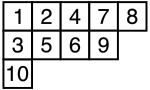
\includegraphics[width=\textwidth]{content/mathematics/young-tableaux.png}
\end{minipage}
}
\hfill
\fbox{
\begin{minipage}{0.06\textwidth}
Hooks:
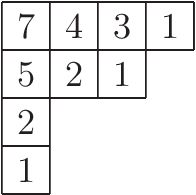
\includegraphics[width=\textwidth]{content/mathematics/hook-length-tableau.jpg}
\end{minipage}
}

\subsection{Burnside's lemma}

Let $G$ be a finite group that acts on a set $X$.

The \textit{orbit} of an element $x$ in $X$ is the set of elements
in $X$ to which $x$ can be moved by the elements of $G$.
The orbit of $x$ is denoted by $G \cdot x$:
 $$G \cdot x = \{g \cdot x\, |\, g \in G\}.$$
For each $g$ in $G$, let $X^g$ denote the set of elements
in $X$ that are fixed by $g$ (also said to be left invariant by $g$),
that is, $X^g = \{ x \in X\, |\, g \cdot x = x \}$.
Burnside's lemma asserts the following formula for the number of orbits,
denoted $|X/G|$:
$$|X/G| = \frac{1}{|G|} \sum_{g \in G} |X^g|.$$

\subsection{Graphs}

\subsubsection{Prüfer sequence}
At step $i$, remove the leaf with the smallest label and set the $i$-th 
element of the Prüfer sequence to be the label of this leaf's neighbour.
The Prüfer sequence of a labeled tree is unique and has length $n - 2$.

The number of spanning trees of $K_n$ is $n^{n - 2}$.\\
The number of spanning trees of $K_{L, R}$ number is $L^{R - 1} \cdot R^{L - 1}$.

Let $T_{n, k}$ be the number of labelled forests on $n$ vertices with $k$ connected components, 
such that vertices $1, \dots, k$ all belong to different components. 
$T_{n,k} = k \cdot n^{n - k - 1}$.

The number of spanning trees in a complete graph $K_{n}$ with the fixed degrees
$d_{i}$ is equal to:
$ \frac{(n - 2)!}{\prod(d_i - 1)} $

For a forest graph with connected components of sizes $s_0, \dots, s_{k - 1}$, 
the number of ways to add edges to make a spanning tree is equal to:
$ n^{k - 2} \cdot \prod s_i$

\subsubsection{Chromatic polynomial}
For a graph $G$, $\chi(G, \lambda) = \chi(\lambda)$ counts the number of its vertex $\lambda$-colorings.
There is a unique polynomial $\chi(\lambda)$. Deletion-contraction:
\begin{itemize}
\item The graph $G/uv$ is obtained by merging $u$ and $v$.
\item The graph $G - uv$ is obtained by deleting the edge $uv$.
\item $\chi(G, \lambda) = \chi(G - uv, \lambda) - \chi(G/uv, \lambda)$. 
\end{itemize}

\begin{tabular}{|c|c|}
\hline
$G$ is tree & $\chi(\lambda) = \lambda(\lambda - 1)^{n - 1}$ \\
\hline
$G$ is cycle $C_n$ & $\chi(\lambda) = (\lambda - 1)^n + (-1)^n(\lambda - 1)$\\
\hline
\end{tabular} 
 
\textbf{Proposition} $\chi(\lambda)$ is equal to the number of pairs $(\sigma, O)$, 
where $\sigma$ is any map $\sigma : V \rightarrow \{1, \dots, \lambda\}$ and $O$ is an orientation of $G$, 
subject to the two conditions:
\begin{itemize}
\item The orientation $O$ is acyclic.
\item If $u \rightarrow v$ in $O$, then $\sigma (u) > \sigma (v)$.
\end{itemize}

Define $\overline{\chi}(\lambda)$ to be the number of pairs $(\sigma, O)$, 
where $\sigma$ is any map $\sigma : V \rightarrow \{1, \dots, \lambda\}$ and $O$ is an orientation of $G$, 
subject to the two conditions:
\begin{itemize}
\item The orientation $O$ is acyclic.
\item If $u \rightarrow v$ in $O$, then $\sigma (u) \ge \sigma (v)$.
\end{itemize}

\textbf{Theorem} Suppose that $|V| = n$. Then for all non-negative integers $\lambda$ holds:
$$\overline{\chi}(\lambda) = (-1)^n \chi(-\lambda)$$

\textbf{Corollary} $(-1)^n \chi(G, -1)$ is equal to the number of acyclic orientations of $G$.

\subsubsection{Kirchhoff's theorem}

Let $G$ be a finite graph, allowing multiple edges but not loops.

The laplacian matrix $L$ of $G$ is the $n \times n$ matrix whose
$(i, j)$-entry $L_{i j}$ is given by
\begin{displaymath}
L_{i j} = \left\{ \begin{array}{ll}
-m_{i j}, & \textrm{if $i \ne j$, $m_{i j}$ edges between $v_i$ and $v_j$, } \\
\deg(v_i), & \textrm{if $i = j$.}
\end{array} \right.
\end{displaymath}

Let $L_0$ denote $L$ with the $i$-th row and column removed for any $i$.
Then for a connected graph, $\det(L_0)$ equals the number of spanning trees of $G$.
